{
\chapter[Image identification from brain activity]{Image identification\\from brain activity}
\label{ch:imageid}
\renewcommand{\chapterpath}{includes/image-id}
%
\begin{contributors}
    Wietske Zuiderbaan, Ben M. Harvey and Serge O. Dumoulin are the authors of the article upon which this work builds. Wietske and Serge supervised the work during my internship at their lab. Akhil Edadan and Peter K{\"onig} participated in the discussions.
\end{contributors}
%
\begin{outreach}
    \item \textit{Saliency and the population receptive field model to identify images from brain activity.} \textbf{Alex Hern{\'a}ndez-Garc{\'i}a}, Wietske Zuiderbaan, Akhil Edadan, Serge O. Dumoulin, Peter K{\"o}nig. Annual Meeting of the Visual Sciences Society (VSS, poster presentation), 2019.
\end{outreach}
%
The goal of computational neuroscience is to understand the mechanisms and principles by which the brain yields behaviour and cognition. One of the approaches to deepen our understanding of the brain is to develop models that can make predictions about brain activity. These methods, sometimes referred to as \textit{brain}/\textit{mind reading}, not only have some practical applications, but they also provide insights about the underlying neural processes that enable the prediction \citep{tong2012mindreading}. 

One particular example for the study of the visual system is the identification of presented images from brain imaging recordings, such as fMRI, in the visual cortex. While a successful approach to this challenge is to use statistical models that can learn activations patterns from a set of recordings \citep{kay2008imageid}, an alternative approach is to rely on biologically inspired encoding models. A recent proposal of this type showed that it is possible to identify the presented stimulus from a set of natural images by comparing the measured activity on areas V1, V2 and V3 with a predicted response profile encoded by the low-parametric population receptive field (pRF) model and contrast information from the images \citep{zuiderbaan2017imageidentification}. In the work presented in this chapter, we follow up this methodology by studying the predictive power of salience information from the images---instead of contrast---combined with the pRF model, and extend the analysis to higher visual areas: V1, V2, V3, hV4, LO12 and V3AB\footnote{This work was carried out during a 2-months internship at the Spinoza Centre for Neuroimaging in Amsterdam, in early 2018, supervised by Dr. Wietske Zuiderbaan and Professor Serge Dumoulin. Besides the potential scientific interest of the work, which was presented as a poster at the 19th Annual Meeting of the Vision Sciences Society (VSS), the internship was part of the training programme of my PhD fellowship, a Marie Skłodowska-Curie Innovative Training Network. A requirement of the programme is to carry out interdisciplinary internships at laboratories that are part of the partnership. As an additional contribution of my internship, I developed interactive visualisation tools in Python to better interpret the kind of data used in this project which became part of the laboratory's repository.}.

\section{Methods}
\label{sec:imageid-methods}
The goal of this study was to assess whether the salience information of images is predictive of brain activations in the visual cortex elicited by the visualisation of natural images. As a follow-up study of the work by \citet{zuiderbaan2017imageidentification}, a significant part of the methodology is borrowed from the first publication and, in particular, the neuroimaging data is the same. In this section, we will outline the most relevant aspects of the methodology that is not original of this work and refer to the original publication for further details, so as to focus on the aspects that are novel here.

\subsection{Visual stimuli}
As a data set of images we used a subset of 45 images from the Berkeley Segmentation Dataset and Benchmark \citep{martin2001berkeley}, which was already used in some of the experiments by \citep{zuiderbaan2017imageidentification}. The data set was processed such that the resulting images had a resolution of $538\times538$ pixels and were applied a circular fading mask. The set of 45 images as they were used in the experiments are shown in Figure~\ref{fig:imageid-berkely}.

\begin{figure}[htb]
  \begin{center}
    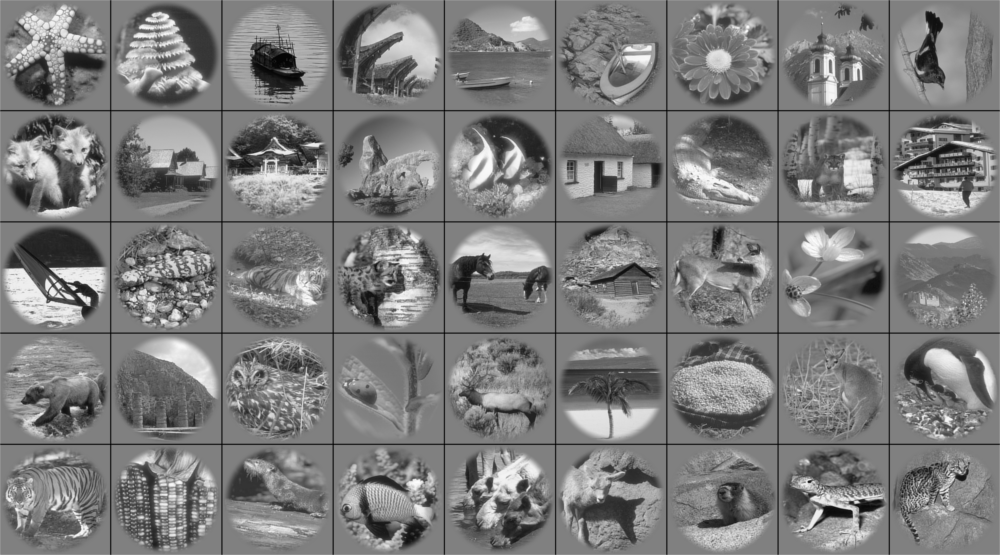
\includegraphics[width = \linewidth]{\imgpath/berkeley.png}
  \end{center}
  \caption{The set of 45 natural images used in the experiments}
\label{fig:imageid-berkely}
\end{figure}

\subsection{Functional imaging}
\label{sec:imageid-functional_imaging}
The brain activations in the visual cortex were acquired in a neuroimaging study with functional magnetic resonance imaging (fMRI), carried out originally for the work presented by \citet{zuiderbaan2017imageidentification}. Therefore, the details can be found in that first article and here we will summarise the most relevant information: Two participants (one female; ages 28-38 years) took part in the fMRI study, were their brain responses to the natural images were collected. Each image was shown 18 times for a duration of 300 ms, with a radius of $5.5^{\circ}$ from the participant point of view. The neural response at each cortical location (voxel) was obtained through standard GLM-analysis \citep{friston1995fmrianalysis}: each voxel was summarised by the t-value of the fit between the predicted time series---the stimulus presentation convolved with the hemodynamic response function---and the measured BOLD signal.

In addition to the voxel responses to each stimulus, the optimal parameters of the population receptive field (pRF) model were estimated for each participant using the standard approach described by \citet{dumoulin2008prf}: For each voxel, the model estimates the position of the receptive field $(x, y)$ and the size $\sigma$ (standard deviation) using a Gaussian kernel. The parameters of the pRF were estimated using conventional contrast-defined moving-bar apertures with natural image content from images of the same data set but distinct from the set of 45 images used in the image identification experiments.

\citet{zuiderbaan2017imageidentification} analysed areas V1, V2 and V3 of the visual cortex as regions of interest. Here, we extended the analysis to higher visual areas: on the lateral occipital complex (LO-1 and LO-2: LO12), on the ventral occipital (hV4) and on the dorsal occipital (V3A and V3B: V3AB) \citep{wandell2007visualfield}. See Figure~\ref{fig:imageid-visual_field_maps} for an illustration of the regions of interest in the human visual cortex.

\begin{figure}[htb]
  \begin{center}
    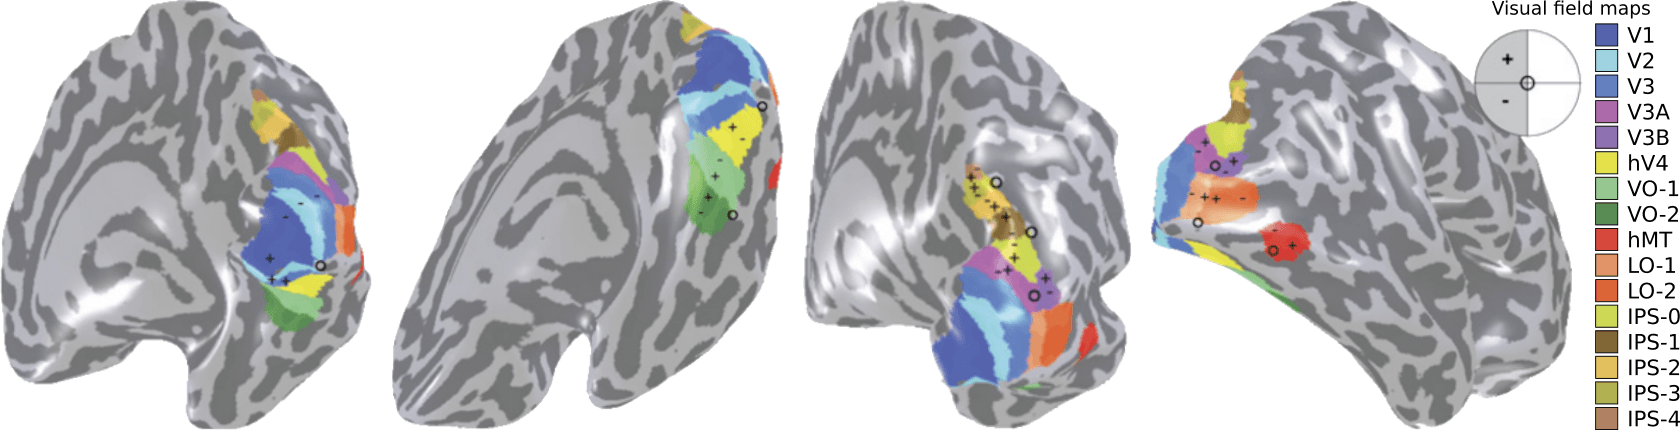
\includegraphics[width = \linewidth]{\imgpath/visual_field_maps.png}
  \end{center}
  \caption{Adapted from \citep{wandell2007visualfield} with permission from the authors: Visual field maps in the human visual cortex. In our analyses, V3A and V3B were considered a single region of interest (V3AB), and so were LO-1 and LO-2 (LO12).}
\label{fig:imageid-visual_field_maps}
\end{figure}

\subsection{Salience and contrast maps}
One of the goals of this work was to contrast the correlation of salience maps with the activations in the visual cortex, and the predictive ability of contrast maps---calculated as the root mean squared contrast---which was assessed in the original article by \citet{zuiderbaan2017imageidentification}. The choice of contrast is motivated by the evidence that the early visual cortex responds strongly to differences in contrast \citep{boynton1999contrast, olman2004contrast}. However, the visual cortex certainly responds to other properties of the stimuli and hence the interest in studying salience.

In order to analyse the correlation of salience with the activations in the visual cortex, we computed the salience maps of each image using two distinct salience models. One of the models is  DeepGaze II\footnote{Note that in Chapter~\ref{ch:globsal} we also used DeepGaze to analyse whether our proposed global salience was related or independent from the local salience properties of images, proposed by \citet{kuemmerer2016deepgaze}. DeepGaze II---for better readability, in what follows we will simply refer to it as DeepGaze---is a model that uses the features extracted by a deep neural network, VGG \citep{simonyan2014vgg}, trained on image object categorisation tasks as inputs to a 4-layer readout neural network optimised for salience prediction}, the then state-of-the-art salience model for various metrics. The second model is ICF, which stands for Intensity Contrast Features, proposed by \citet{kuemmerer2017icfdeepgaze}. ICF is trained on the same readout neural network as DeepGaze, but instead of using the VGG features, the input to the network are 5 intensity and 5 contrast feature maps.

Our choice of salience models, out of the many models proposed in the vast literature on image salience, was motivated by various reasons. First of all, we chose DeepGaze as it was the state-of-the-art model in various metrics of image salience evaluation \citep{kuemmerer2016deepgaze} and considering a model that accurately predicts the salient regions of images is also desirable for studying how salience information is encoded in the visual cortex. Nonetheless, as we have discussed in Chapter~\ref{ch:globsal}, visual attention is a complex brain mechanism and salience maps capture different aspects of it. For instance, we have discussed how visual attention can be guided by both bottom-up factors, as well as top-down factors and higher-level features. This motivated the inclusion of a model that is limited to lower-level---intensity and contrast---features, in this case ICF. The fact that DeepGaze and ICF share part of the architecture facilitates the comparisons. 

Interestingly, \citet{kuemmerer2017icfdeepgaze} analysed and compared the properties of DeepGaze and ICF, and found that while DeepGaze generally outperformed ICF in terms of the evaluation metrics used to assess salience models, ICF was more accurate in a large number of images. In particular, DeepGaze succeeds at predicting salient regions associated with higher-level factors such as objects and faces, while ICF was superior in the cases were fixations are driven by, for instance, high contrast. By way of illustration, in Figure~\ref{fig:imageid-sample_maps} we show the DeepGaze and ICF salience maps of three images from the data set, as well as their contrast maps, which were used in the original study.

\begin{figure}[htb]
  \begin{center}
    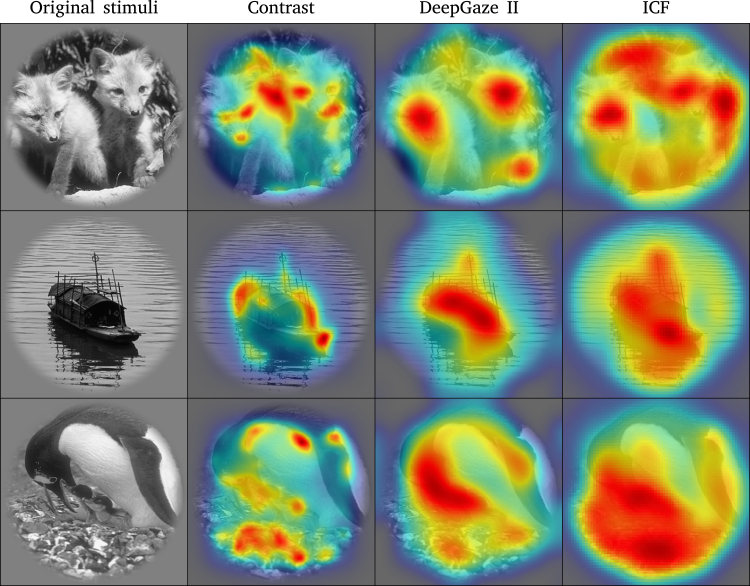
\includegraphics[width = 0.8 \linewidth]{\imgpath/sample_maps.png}
  \end{center}
  \caption{Contrast, DeepGaze II and ICF maps of three images of the data set.}
\label{fig:imageid-sample_maps}
\end{figure}

\subsection{Brain response predictions}
To assess the correspondence between the salience and contrast maps and the brain activations, we first calculated a prediction response profile of every image as the summed overlap of the map with the pRF weighting function of each cortical location, normalised by the total volume of the pRF: 

\begin{equation}
\label{eq:imageid-pred}
    p = \frac{\sum_{i=1}^{N}w_i S_i}{\sum_{j=1}^{M}w_j}
\end{equation}
%
where $S_i$ denotes the value of the feature map $S$---either DeepGaze, ICF or contrast---normalised as a probability distribution, at pixel $i$; $N$ is the number of pixels within the window of the pRF and $M$ is the total number of pixels in the stimulus area. $w_i$ is the pRF weighting function, whose parameters were obtained as described in Section~\ref{sec:imageid-functional_imaging} and in \citep{zuiderbaan2017imageidentification} in more detail:

\begin{equation}
\label{eq:imageid-prf}
    w_i = \exp\left(-\frac{(x_i-x_c)^2+(y_i-y_c)^2}{2\sigma^2}\right)
\end{equation}
%
where $x_i$ and $y_i$ are the locations of pixel $i$; $x_c$ and $y_c$ are the centre of the pRF in the visual field; and $\sigma$ is the size of the Gaussian kernel of the pRF. Note that in \citep{zuiderbaan2017imageidentification} this is the procedure used to compute the predictions of synthetic images, while for natural images a different method was used, which was specific for the way the contrast information was obtained. Here, we use this method, since we can generalise the prediction $p$ in Equation~\ref{eq:imageid-pred} to any feature map $S$---DeepGaze, ICF or contrast.

\subsection{Evaluation metrics}
Let us formally express the measurements and predictions taking all variables into account---feature maps, areas, images, voxels---in order to describe the evaluation metrics we used in our analysis. First note that, as in the original study by \citet{zuiderbaan2017imageidentification}, we only considered for the analysis the voxels with positive t-value, pRF eccentricity values within $0.5\text{---}4.5^{\circ}$ and pRF variance explained larger than 55 \%. For every image $k$ and every visual area $A$ studied---V1, V2, V3, hV4, LO12 and V3AB---we have a \textit{measured} response profile 
%
\[
    \mathbf{m}_{k}^{A} = m_{k, 1}^{A}, \ldots, m_{k, D_A}^{A}
\]
%
where $D_A$ is the number of (\textit{valid}) voxels in area $A$. Correspondingly, we have the \textit{predicted} response profiles for every image $k$, every visual area $A$ and by every feature map $S$, that is DeepGaze, ICF and contrast:

\[
    \mathbf{p}_{k}^{A, S} = p_{k, 1}^{A, S}, \ldots, p_{k, D_A}^{A, S}
\]
%
where every $p_{k, v}^{A, S}$ is computed as in Equation~\ref{eq:imageid-pred}. As a similarity metric we compute the Pearson correlation between measured responses and predicted profiles. We will denote by $r_{k, l}^{A, S}$, or simply $r_{k, l}$ abusing notation, to the correlation between the measured response of image $k$, $\mathbf{m}_{k}^{A}$, and the predicted profile of image $l$, $\mathbf{p}_{l}^{A, S}$: 

\begin{equation}
\label{eq:imageid-correlation}
	r_{k, l}^{A, S} = corr(\mathbf{m}_{k}^{A}, \mathbf{p}_{l}^{A, S})
\end{equation}

In order to assess the image identification accuracy we simply considered a correct identification if $r_{k, k} > r_{k, l}$, $\forall~k \neq l$. Additionally, as a more informative metric, we combined the correlation values into a confidence score that represents how hard it is to distinguish the actual presented image $k$ from the other candidate images in the data set, based on the correlation values:

\begin{equation}
\label{eq:imageid-confidence}
c_k^{A, S} = r_{k, k}^{A, S} - \frac{1}{K}\sum_{l=1}^{K}r_{k, l}^{A, S}
\end{equation}

Finally, in order to have a compact measure to compare the predictivity of the different feature maps on every visual area, we also performed a representational similarity analysis\footnote{In Chapter~\ref{ch:daugit}, we also used representational similarity analysis to compare the features learnt by artificial neural networks and the representations measured in the inferior temporal cortex.} (RSA) \citep{kriegeskorte2008rsa}. In order to perform RSA, we constructed representational dissimilarity matrices (RDM) for both the measured responses and the predicted profiles, $M_{k, l}^{A}$ and $P_{k, l}^{A, S}$ respectively, where each entry $(k, l)$ of the matrices is 1 minus the Pearson correlation between the profile for image $k$ and image $j$. In this case, the correlation is not computed between the measured and the predicted profiles, but between two measured responses for $M_{k, l}$ and two predicted profiles for $P_{k, l}$. Thus, the RDMs are symmetric and the values in the diagonals are zero. As a summary metric to compare $M$ and $P$ we computed the Kendall correlation.

\section{Results and discussion}
\label{sec:imageid-results}
We first analyse the distribution of the confidence of the predictions for each model---feature map---and visual area, shown in Figure~\ref{fig:imageid-boxplot_confidence}. Although the results are complex and not highly consistent, several interesting conclusions can be drawn. First, we observe that the identification ability of all models is best on V1 and decreases in higher visual areas. This was observed by \citep{zuiderbaan2017imageidentification} too, who analysed V1, V2 and V3; and we here confirmed it, although we had hypothesised that salience maps might be more discriminative in higher visual areas. Unfortunately, it is not possible to conclude from our results that contrast and salience are less predictive of the activations in higher visual areas because this result could be also explained by the increased pRF sizes \citep{smith2001rfsizes}. In what follows, our analysis will focus in the earlier areas---V1, V2, V3 and, to a lesser extent, hV4---where the identification performance is better and the differences between models larger.

\begin{figure}[htb]
  \begin{center}
    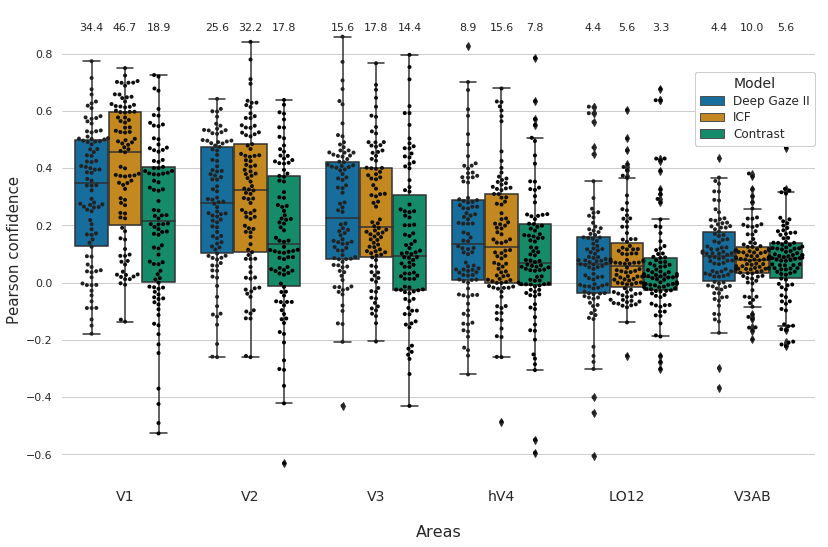
\includegraphics[width = \linewidth]{\imgpath/boxplot_confidence.png}
  \end{center}
  \caption{Distribution of the confidence values (see Equation~\ref{eq:imageid-confidence}) for every feature map and visual area. Each black dot corresponds to the confidence of the prediction for one image $k$, from the data of one of the experimental participants. The numbers over each box represent the identification accuracy (as a percentage).}
\label{fig:imageid-boxplot_confidence}
\end{figure}

Second, the most relevant observation is that both salience models, DeepGaze and ICF, seem more predictive of the measured activations in the visual cortex than the contrast maps of the images. A significant difference can be observed in both the median of the distribution of the confidence values and in the identification accuracy, shown over each box. For instance, the identification accuracy on V1 using DeepGaze and ICF maps is 34.4 \% and 46.7 \% respectively, while it is below 20 \% using contrast\footnote{In the first publication by \citet{zuiderbaan2017imageidentification} the prediction model for natural images using contrast is computed differently and the evaluation procedures are not the same, hence the results differ slightly to the ones presented here. Nonetheless, in our study we analysed both methods and the results are qualitatively very similar. We here present the results using contrast maps, since the method is identical for salience maps.}.

Although image identification from brain activity has been shown before \citep{kay2008imageid}, the identification performance of the methods presented here is remarkable due to the simplicity of the model. The main differences between this pRF-based method and the model presented by \citet{kay2008imageid} were reviewed by \citet{zuiderbaan2017imageidentification}, but most importantly, note that here we estimated only 3 pRF parameters for each voxel---location and size of the receptive field---which were obtained from the fMRI recordings of a standard pRF session: responses to conventional moving-bar apertures during about half an hour. Then, the 3 pRF parameters are combined with the contrast or salience maps of the images to predict the activity of each voxel. In contrast, \citet{kay2008imageid} recorded the activations to 1,750 natural images (about 5 hours of scanning time) to fit a Gabor-Wavelet-Pyramid model with 2,730 parameters per voxel. Summarised, image identification with the pRF model requires a short scanning time and does not require training a model with brain activations towards natural image. Thus, it can be easily applied to any other image.

The fact that identifying natural images from brain activity using salience maps is more accurate than using contrast information from the images tells us that the image salience \textit{under} the receptive field of each voxel is more discriminative than the contrast. This may come as a surprise, since the early visual cortex is well known to respond strongly to differences in contrast \citep{boynton1999contrast, olman2004contrast}. Salience maps also certainly contain contrast information, in our analysis especially the maps obtained with the ICF model, but not only. Therefore, our results can be interpreted as additional evidence of the activations in the early visual cortex being shaped by multiple factors, likely top-down influences \citep{treue2003salience}.

\begin{figure}[htb]
  \begin{center}
    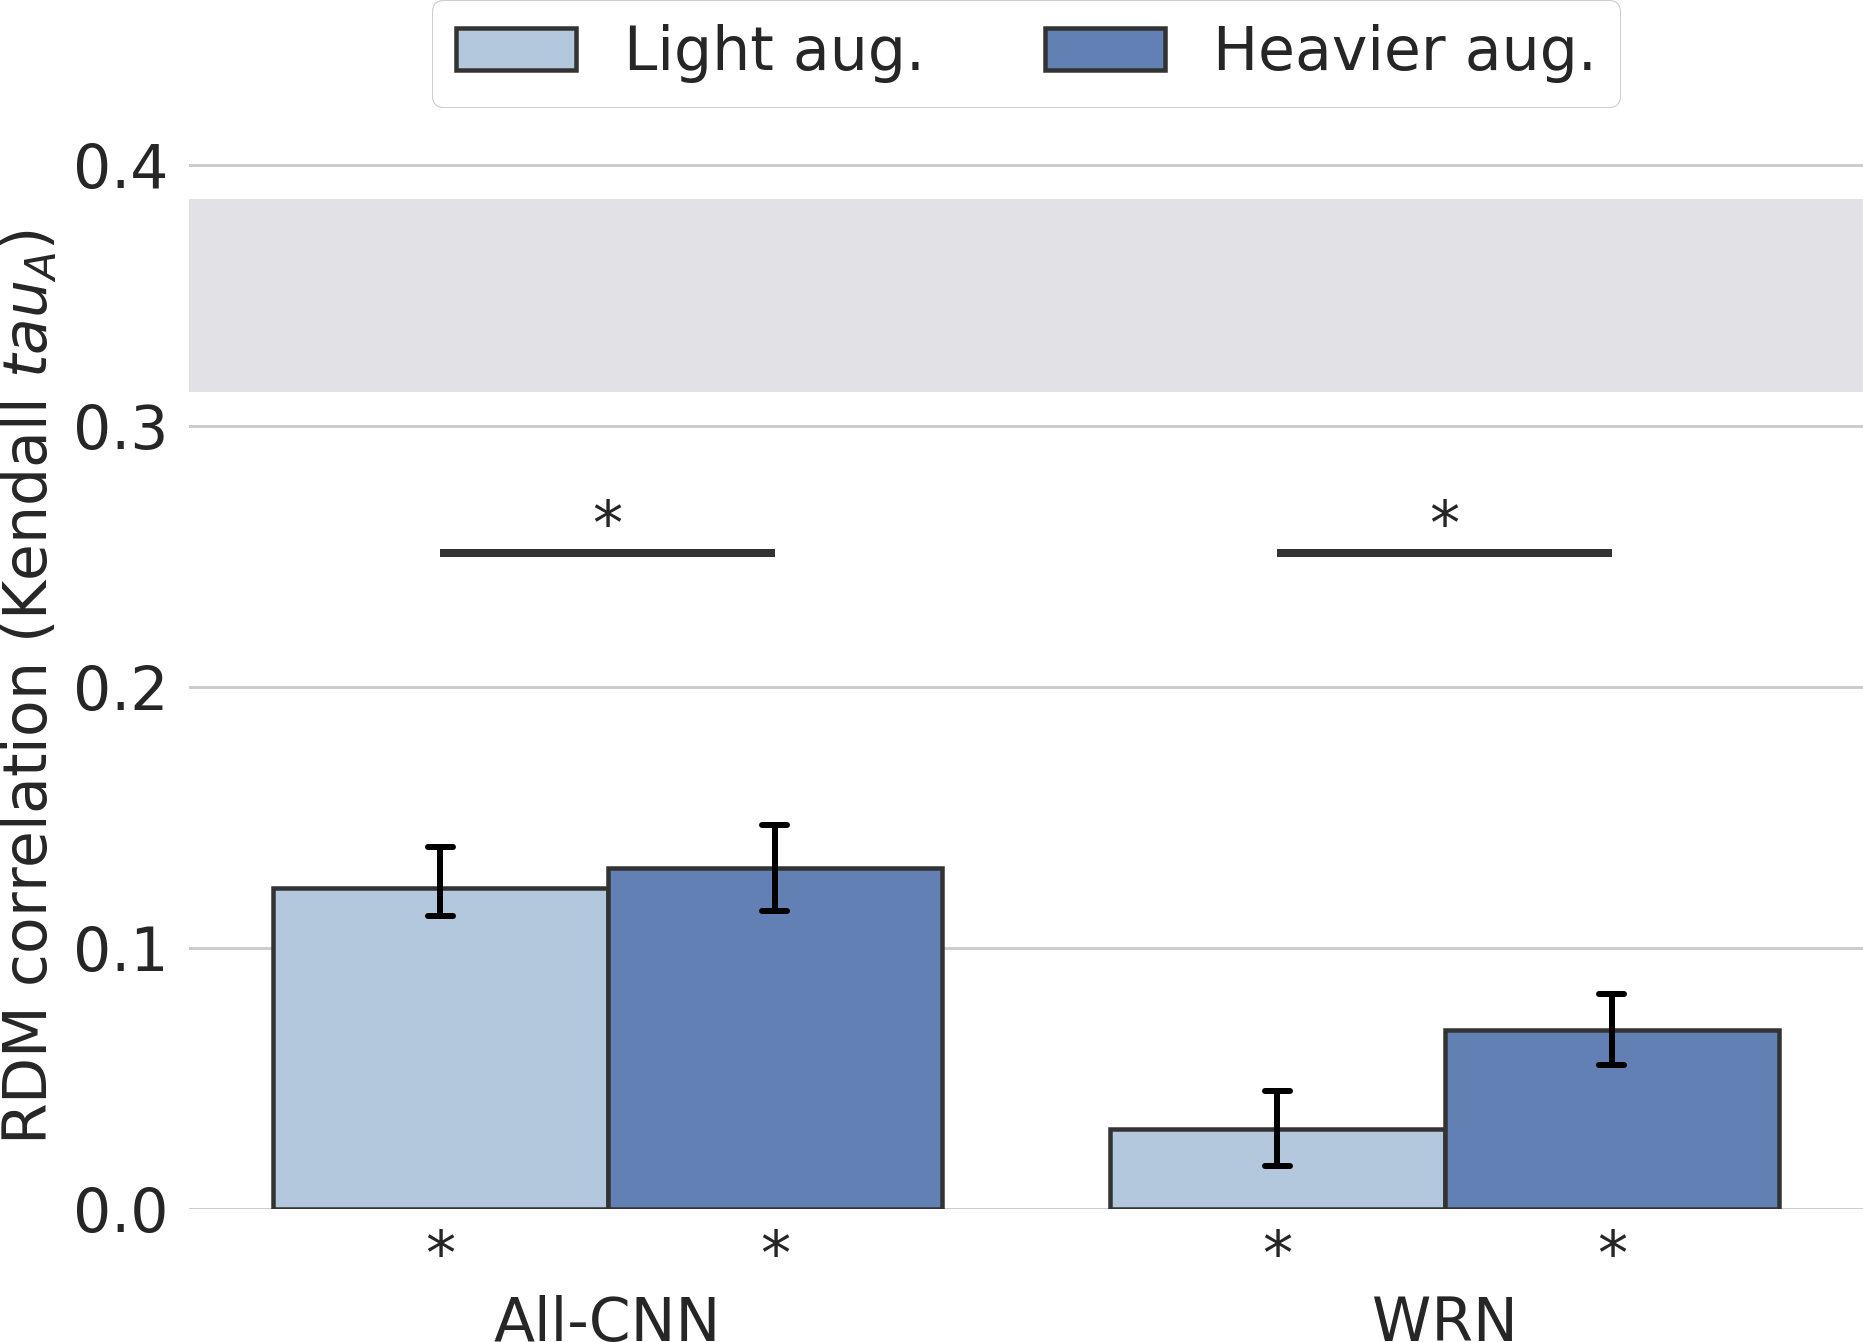
\includegraphics[width = \linewidth]{\imgpath/kendall.png}
  \end{center}
  \caption{Results of the representational similarity analysis (RSA): Kendall correlation between the representational dissimilarity matrices of the measured responses and the predicted profiles. The error bars correspond to the variation across experimental participants.}
\label{fig:imageid-kendall}
\end{figure}

Another interesting conclusion derives from the comparison between the two salience models analysed. Recall that DeepGaze computes the salience map by first extracting features through a deep neural network trained on image object recognition tasks. Therefore, these features likely contain high-level information such as face and object detectors and the model is particularly accurate at spotting salience driven by such factors, as reflected in Figure~\ref{fig:imageid-sample_maps}. On the contrary, ICF does not extract high-level features but is restricted to intensity and contrast features. Here, we found that image identification is more accurate by using ICF than DeepGaze salience maps. While this is observable in Figure~\ref{fig:imageid-boxplot_confidence}, we additionally perform a representational similarity analysis (RSA) to derive a compact metric of the ability of each model to discriminate the brain activations of each image. We present these results in Figure~\ref{fig:imageid-kendall}, which confirms the conclusion that ICF is more discriminative than DeepGaze in the earlier visual areas.

One more way to visualise the superiority of ICF at predicting brain activations in the early visual cortex is by directly analysing the correlation matrices. In Figure~\ref{fig:imageid-corr}, we plot the correlation matrices of each model on V1, where each element in the matrix encodes the correlation between the measured responses of one image (rows) and the predicted profile of another image (columns), as in Equation~\ref{eq:imageid-correlation}. Note that a correct identification occurs when the element in the diagonal---correlation between measured and predicted profile of the same image---has the highest value in the row. Visually, it becomes apparent that the diagonal in the ICF model has higher values and is better discriminated from the rest of the matrix, than in the DeepGaze model, and yet more in the contrast model. In view of these results, we conclude that image salience is more predictive of the brain activity in the early visual cortex than contrast information, and hypothesise that ICF may be more accurate than DeepGaze because the salience of the latter is driven by high-level information that may not correlate with the activity in the early areas of the visual cortex.

\begin{figure}[htb]
  \begin{center}
    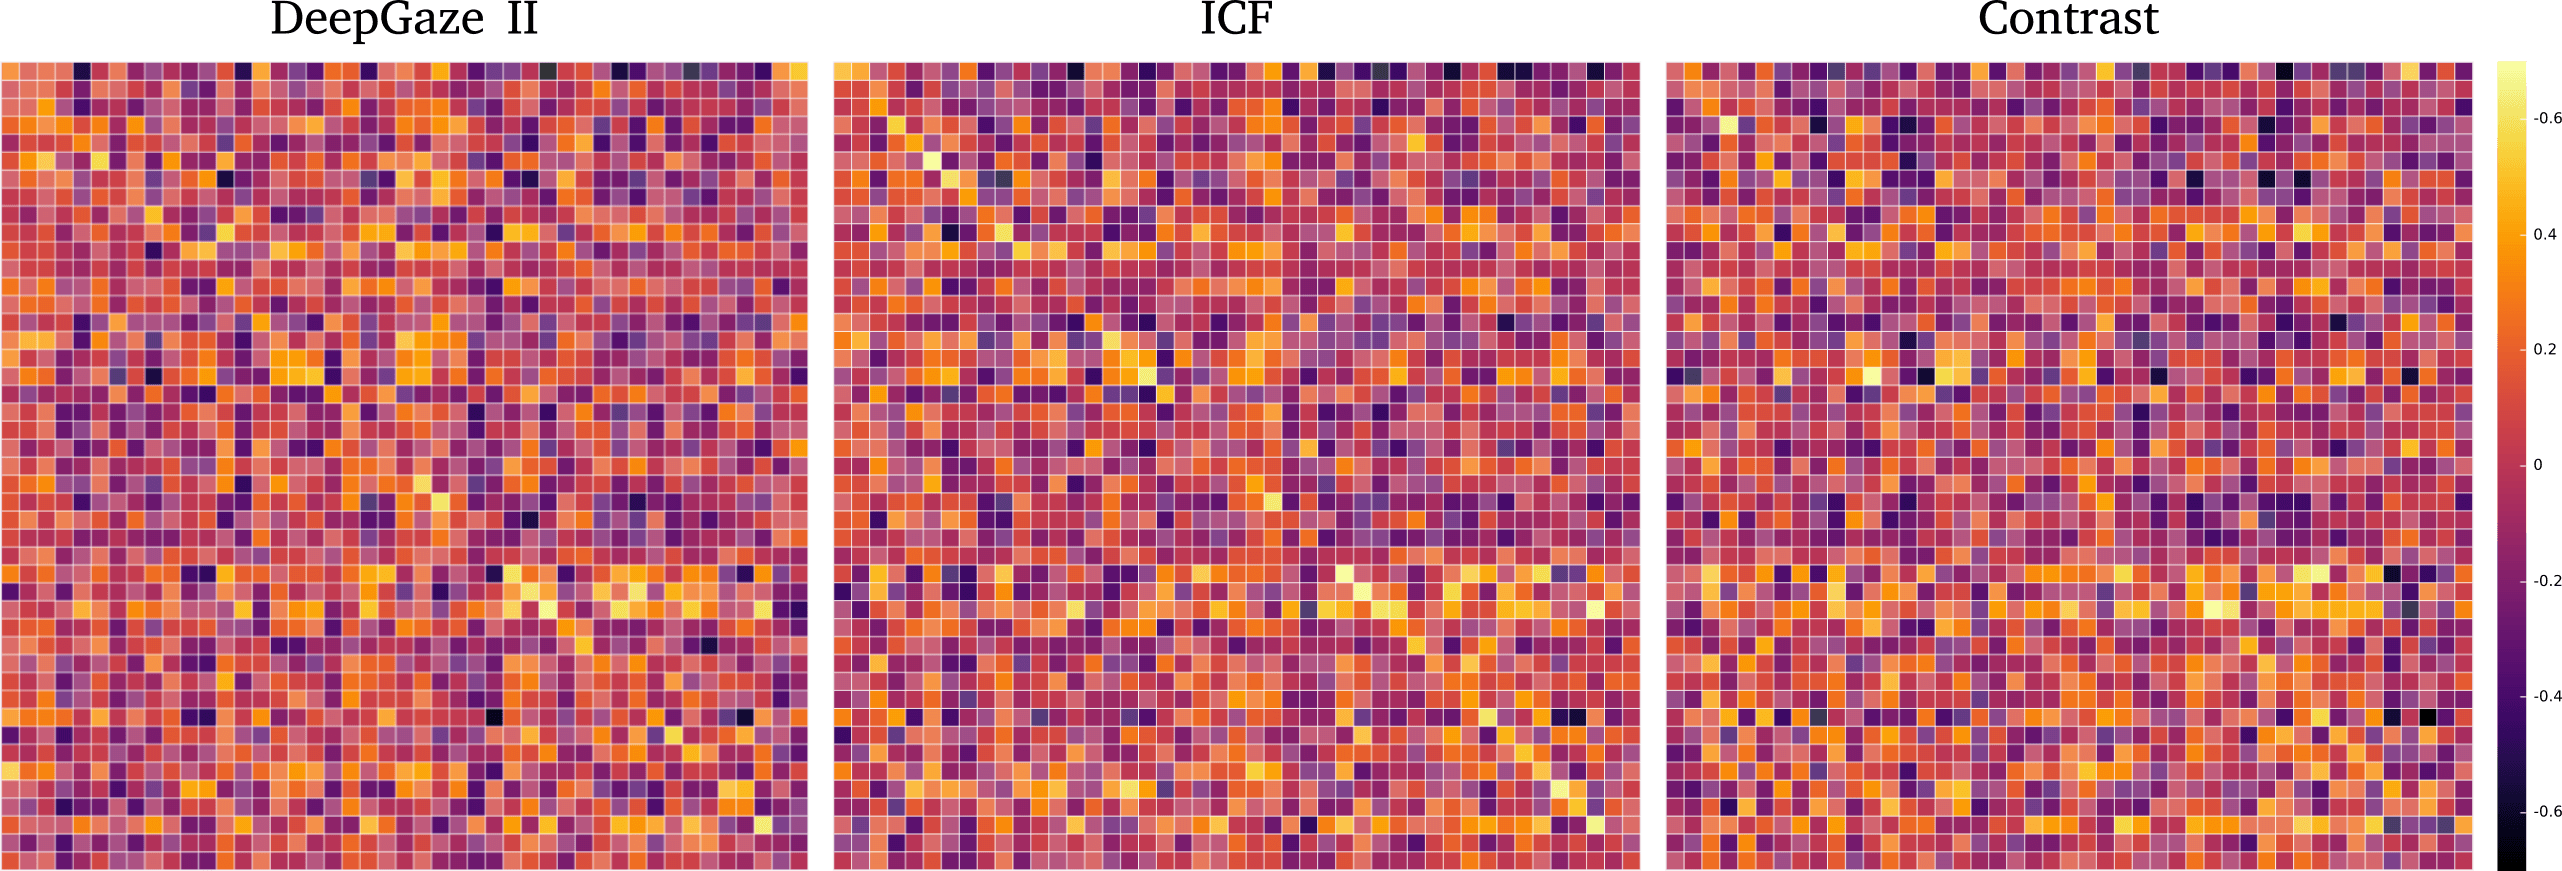
\includegraphics[width = \linewidth]{\imgpath/corr_matrices_v1.png}
  \end{center}
  \caption{Correlation matrices of the three models for the predictions in visual area V1. Each entry $(i, j)$ of the matrices represent $r_{i, j}^{V1, S} = corr(\mathbf{m}_{i}^{V1}, \mathbf{p}_{j}^{V1, S})$.}
\label{fig:imageid-corr}
\end{figure}

The data we obtained from the predictions allows for multiple levels of analysis, since there are several factors at play: three feature maps, six visual areas, two subjects, etc. During the two-months internship in which this project was carried out, I developed multiple interactive visualisation using Bokeh\footnote{Bokeh is an interactive visualisation library for Python: \href{https://bokeh.org/}{www.bokeh.org}} and the interactive functionality of Jupyter notebooks. Interactive visualisation provides insights that are hardly accessed otherwise and is useful to guide the more systematic, conventional, statistical analyses. In particular, it can be used to analysed the results at different levels of analysis and to look into specific details or data points. Some examples are shown in Figure~\ref{fig:imageid-interactive_visualisation}.

\begin{figure}[htb]
  \centering
  \begin{subfigure}{0.32 \linewidth}
      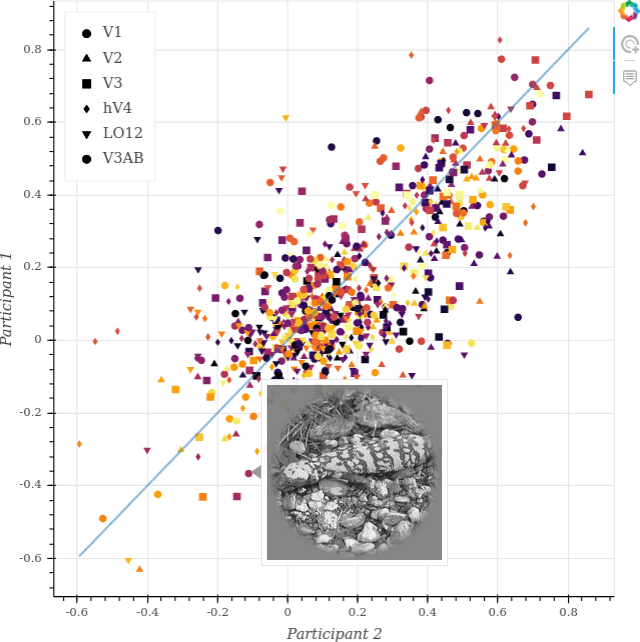
\includegraphics[width = \linewidth]{\imgpath/interactive_vis_participants_all.png}
      \label{fig:imageid-participants_all}
  \end{subfigure}
  \begin{subfigure}{0.32 \linewidth}
      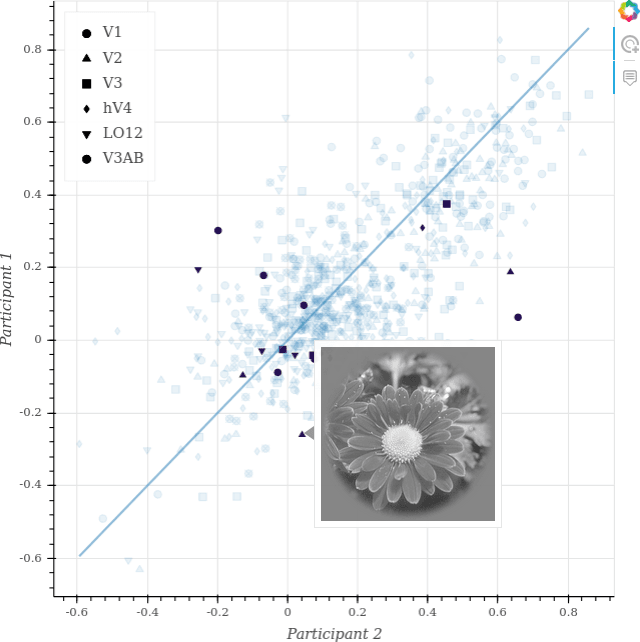
\includegraphics[width = \linewidth]{\imgpath/interactive_vis_participants_specific.png}
      \label{fig:imageid-participants_specific}
  \end{subfigure}
  \begin{subfigure}{0.32 \linewidth}
      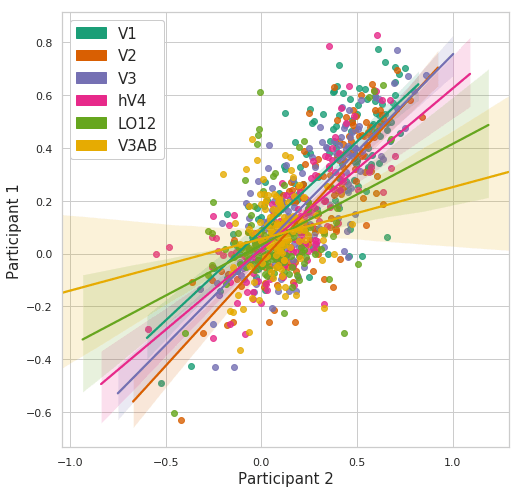
\includegraphics[width = \linewidth]{\imgpath/participants.png}
      \label{fig:imageid-participants_fit}
  \end{subfigure}
  \\
  \begin{subfigure}{\linewidth}
      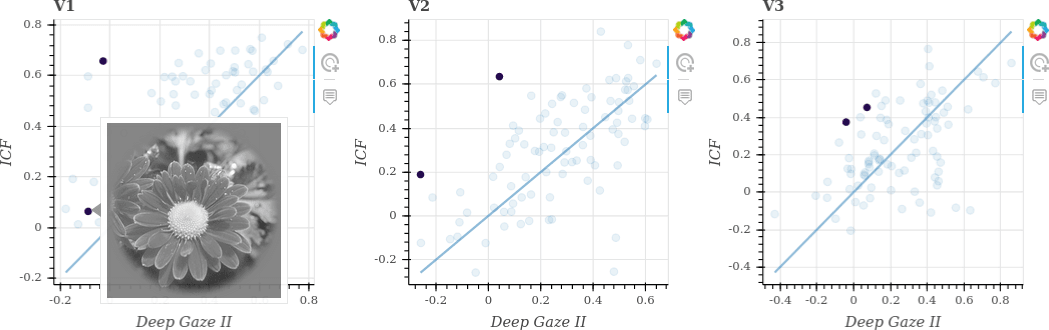
\includegraphics[width = \linewidth]{\imgpath/interactive_vis_icf-vs-dg.png}
      \label{fig:imageid-icf_vs_dg}
  \end{subfigure}
  \caption{Examples of interactive scatter plots of the Pearson confidence (Equation~\ref{eq:imageid-confidence}) to contrast different experimental variables. The interactive plot allows to hover over the data points to visualise the image that they represent and highlight all data points of one image by clicking on them. Bottom row: DeepGaze vs. ICF on areas V1, V2 and V3. Top row: comparison of the confidence values of the predictions from the data of the two experimental participants. From left to right: data from the three models, represented with different shapes for each visual area and different colours for each image; highlight of one image, after clicking on one point; linear fit for each visual area separately.}
  \label{fig:imageid-interactive_visualisation}
\end{figure}

Besides the main conclusions discussed above, some other observations are the following: In general, we found a positive linear correlation in the prediction confidence between the predictions on the data from both participants in areas V1, V2, V3 and hV4 ($r = 0.76, 0.80, 0.78, 0.71$ respectively) and less so in LO12 and V3AB ($r = 0.42, 0.17$), where the predictions were also less confident. We also found a correlation between the predictions across visual areas, that is images that were confidently predicted in V1 were also in V2 ($r = 73$) and in V3 ($r = 0.56$), and the correlation decreases further in higher visual areas, as expected. 

The prediction confidence was also positively correlated between DeepGaze and ICF ($r = 0.58, 0.62, 0.50, 0.58$ in areas V1, V2, V3 and hV4), although with exceptions, that is several images were confidently predicted by ICF but not by DeepGaze, and vice versa. The interactive visualisation was useful to identify and study these cases. Not surprisingly, the correlation was much lower between the salience  and the contrast models. For instance, in V1, the correlation between DeepGaze and contrast and ICF and contrast was $r = 0.25, 0.35$, respectively.

\section{Conclusion}
\label{sec:imageid-conclusion}
In this chapter we have presented the results of a project carried out during a two-months internship at the Spinoza Centre for Neuroimaging in Amsterdam, in which we extended the work presented by \citet{zuiderbaan2017imageidentification}. In particular we analysed the discriminability of salience maps to identify images from brain activity in the visual cortex, using a low-parametric model of the receptive field of the measured cortical locations, the population receptive field (pRF) model \citep{dumoulin2008prf}.

We contrasted the identification performance of two distinct salience models---DeepGaze and ICF--- and the contrast-based model originally presented by \citet{zuiderbaan2017imageidentification} and found that the salience information within the receptive fields of the voxels is more predictive of the brain activity than the contrast information. Furthermore, we observed that ICF, whose salience maps are computed using low-level features, is more predictive than DeepGaze, which encodes high-level information such as salience driven by faces and objects.

Overall, this analysis demonstrates that this simple method of prediction of brain activity using the pRF model can be extended to other types of image information beyond contrast, enabling further analysis. Future work may use this kind of analysis to further understand the computations in the early visual cortex and extend this methodology to other cortical areas.

\chapterbibliography
}

